\documentclass[tikz,border=3mm,multi=tikzpicture]{standalone}
\usepackage{tikz}
\usetikzlibrary{arrows.meta,positioning,shapes.geometric}
\begin{document}
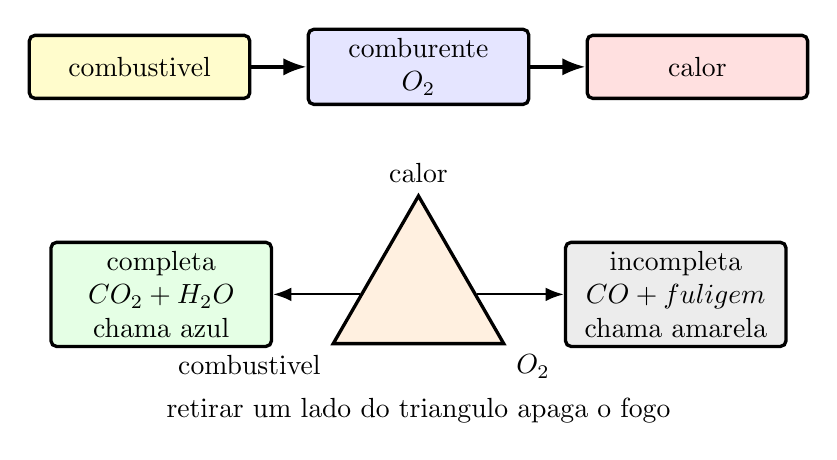
\begin{tikzpicture}[>=Latex,node distance=0.7cm]
  \tikzstyle{box}=[draw,rounded corners=2pt,very thick,minimum width=2.8cm,minimum height=0.8cm,align=center]
  \node[box,fill=yellow!20] (comb) {combustivel};
  \node[box,fill=blue!10,right=0.7cm of comb] (ox) {comburente\\$O_2$};
  \node[box,fill=red!12,right=0.7cm of ox] (calor) {calor};
  \draw[very thick,->] (comb) -- (ox);
  \draw[very thick,->] (ox) -- (calor);
  \node[draw,regular polygon,regular polygon sides=3,minimum size=2.5cm,very thick,fill=orange!12,below=1.1cm of ox] (tri) {};
  \node at (tri.corner 1) [above] {calor};
  \node at (tri.corner 2) [below left] {combustivel};
  \node at (tri.corner 3) [below right] {$O_2$};
  \node[box,fill=green!10,left=1.1cm of tri] (comp) {completa\\$CO_2 + H_2O$\\chama azul};
  \node[box,fill=gray!15,right=1.1cm of tri] (incomp) {incompleta\\$CO + fuligem$\\chama amarela};
  \draw[thick,->] (tri) -- (comp);
  \draw[thick,->] (tri) -- (incomp);
  \node[align=center,below=0.55cm of tri] {retirar um lado do triangulo apaga o fogo};
\end{tikzpicture}
\end{document}
